\documentclass[10pt,tikz]{standalone}
\usepackage[T1]{fontenc}
\usepackage{helvet}
\renewcommand{\familydefault}{\sfdefault}
\usepackage{tikz}
\usetikzlibrary{positioning, fit, calc, shapes.geometric, arrows.meta, backgrounds, decorations.pathreplacing}

\definecolor{emeraldpine}{HTML}{1A4D3E}
\definecolor{harvardcrimson}{HTML}{A51C30}
\definecolor{ethdarkblue}{HTML}{1F407A}
\definecolor{ethpetrol}{HTML}{007A87}
\definecolor{ethbronze}{HTML}{B87333}
\definecolor{ethpurple}{HTML}{5B4B8A}
\definecolor{ink}{HTML}{1A202C}
\definecolor{softink}{HTML}{4A5568}
\definecolor{paleink}{HTML}{A0AEC0}
\definecolor{cardbg}{HTML}{F8FAFC}
\definecolor{shadecolor}{HTML}{F4F6F9}

\begin{document}
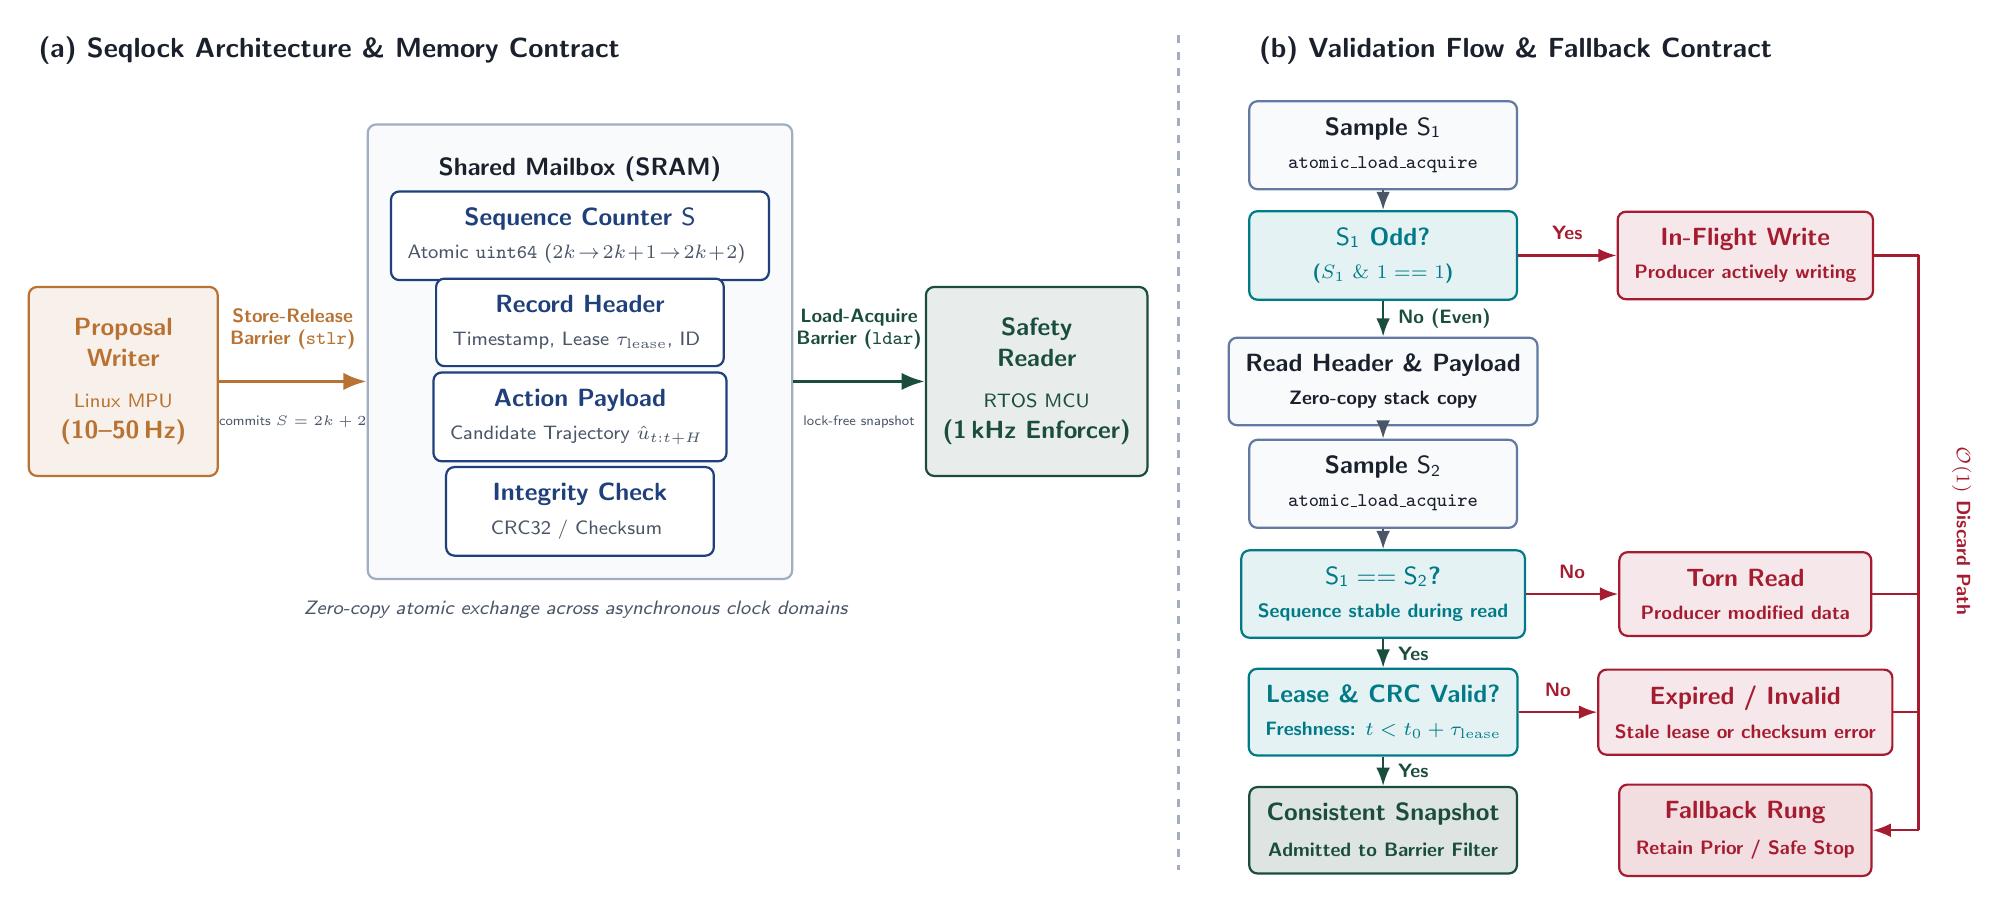
\begin{tikzpicture}[
    >=Latex,
    font=\sffamily,
    box/.style={
        rectangle, 
        rounded corners=3pt,
        draw, 
        thick, 
        align=center, 
        inner sep=6pt, 
        font=\small\bfseries\color{ink}
    },
    propbox/.style={box, draw=ethbronze, fill=ethbronze!10, text=ethbronze},
    authbox/.style={box, draw=emeraldpine, fill=emeraldpine!10, text=emeraldpine},
    databox/.style={box, draw=ethdarkblue, fill=white, text=ethdarkblue},
    warnbox/.style={box, draw=harvardcrimson, fill=harvardcrimson!10, text=harvardcrimson},
    stepbox/.style={box, draw=ethdarkblue!70, fill=cardbg, text=ink},
    decbox/.style={box, draw=ethpetrol, fill=ethpetrol!10, text=ethpetrol},
    arr/.style={->, thick, >=Latex, draw=softink},
    proparr/.style={->, very thick, >=Latex, draw=ethbronze},
    autharr/.style={->, very thick, >=Latex, draw=emeraldpine},
    warnarr/.style={->, thick, >=Latex, draw=harvardcrimson},
]

% ========================================================
% PANEL A: Architecture & Memory Layout
% ========================================================
\node[font=\normalsize\bfseries, text=ink, anchor=west] (titleA) at (-7.0, 0.6) {(a) Seqlock Architecture \& Memory Contract};

% Writer Node
\node[propbox, minimum height=2.4cm, minimum width=2.4cm] (writer) at (-5.8, -3.6) {
    Proposal\\Writer\\[4pt]
    \scriptsize\normalfont\color{ethbronze} Linux MPU\\(10--50\,Hz)
};

% Mailbox Components
\node[font=\small\bfseries, text=ink] (mbox_title) at (0, -0.9) {Shared Mailbox (SRAM)};

\node[databox, minimum width=3.4cm, minimum height=0.7cm] (seq) at (0, -1.75) {
    Sequence Counter $\mathsf{S}$\\[1pt]
    \scriptsize\normalfont\color{softink}Atomic \texttt{uint64} ($2k \!\to\! 2k\!+\!1 \!\to\! 2k\!+\!2$)
};

\node[databox, minimum width=3.4cm, minimum height=0.7cm] (hdr) at (0, -2.85) {
    Record Header\\[1pt]
    \scriptsize\normalfont\color{softink}Timestamp, Lease $\tau_{\mathrm{lease}}$, ID
};

\node[databox, minimum width=3.4cm, minimum height=0.9cm] (payload) at (0, -4.05) {
    Action Payload\\[1pt]
    \scriptsize\normalfont\color{softink}Candidate Trajectory $\hat{u}_{t:t+H}$
};

\node[databox, minimum width=3.4cm, minimum height=0.7cm] (crc) at (0, -5.25) {
    Integrity Check\\[1pt]
    \scriptsize\normalfont\color{softink}CRC32 / Checksum
};

\begin{scope}[on background layer]
    \node[box, draw=paleink, fill=cardbg, fit=(mbox_title)(seq)(hdr)(payload)(crc), inner sep=8pt] (mailbox) {};
\end{scope}

% Reader Node
\node[authbox, minimum height=2.4cm, minimum width=2.4cm] (reader) at (5.8, -3.6) {
    Safety\\Reader\\[4pt]
    \scriptsize\normalfont\color{emeraldpine} RTOS MCU\\(1\,kHz Enforcer)
};

% Barriers & Transfer Arrows A
\draw[proparr] (writer.east) -- (mailbox.west |- writer.east);
\node[above=8pt, font=\scriptsize\bfseries, text=ethbronze, align=center] at ($(writer.east)!0.5!(mailbox.west |- writer.east)$) {Store-Release\\Barrier (\texttt{stlr})};
\node[below=9pt, font=\tiny, text=softink, align=center] at ($(writer.east)!0.5!(mailbox.west |- writer.east)$) {commits $S=2k+2$};

\draw[autharr] (mailbox.east |- reader.west) -- (reader.west);
\node[above=8pt, font=\scriptsize\bfseries, text=emeraldpine, align=center] at ($(mailbox.east |- reader.west)!0.5!(reader.west)$) {Load-Acquire\\Barrier (\texttt{ldar})};
\node[below=9pt, font=\tiny, text=softink, align=center] at ($(mailbox.east |- reader.west)!0.5!(reader.west)$) {lock-free snapshot};

% Footer note for Panel A
\node[font=\scriptsize, text=softink, align=center] at (0, -6.5) {
    \textit{Zero-copy atomic exchange across asynchronous clock domains}
};

% ========================================================
% PANEL DIVIDER
% ========================================================
\draw[draw=paleink, thick, dashed] (7.6, 0.8) -- (7.6, -9.8);

% ========================================================
% PANEL B: Validation Flow & Fallback Contract
% ========================================================
\node[font=\normalsize\bfseries, text=ink, anchor=west] (titleB) at (8.5, 0.6) {(b) Validation Flow \& Fallback Contract};

% Flow Steps
\node[stepbox, minimum width=3.4cm] (step1) at (10.2, -0.6) {
    \textbf{Sample $\mathsf{S_1}$}\\[1pt]
    \scriptsize \texttt{atomic\_load\_acquire}
};

\node[decbox, minimum width=3.4cm] (dec1) at (10.2, -2.0) {
    \textbf{$\mathsf{S_1}$ Odd?}\\[1pt]
    \scriptsize ($S_1 \ \& \ 1 == 1$)
};

\node[warnbox, minimum width=3.2cm] (inflight) at (14.8, -2.0) {
    \textbf{In-Flight Write}\\[1pt]
    \scriptsize Producer actively writing
};

\node[stepbox, minimum width=3.4cm] (step2) at (10.2, -3.6) {
    \textbf{Read Header \& Payload}\\[1pt]
    \scriptsize Zero-copy stack copy
};

\node[stepbox, minimum width=3.4cm] (step3) at (10.2, -4.9) {
    \textbf{Sample $\mathsf{S_2}$}\\[1pt]
    \scriptsize \texttt{atomic\_load\_acquire}
};

\node[decbox, minimum width=3.4cm] (dec2) at (10.2, -6.3) {
    \textbf{$\mathsf{S_1} == \mathsf{S_2}$?}\\[1pt]
    \scriptsize Sequence stable during read
};

\node[warnbox, minimum width=3.2cm] (torn) at (14.8, -6.3) {
    \textbf{Torn Read}\\[1pt]
    \scriptsize Producer modified data
};

\node[decbox, minimum width=3.4cm] (dec3) at (10.2, -7.8) {
    \textbf{Lease \& CRC Valid?}\\[1pt]
    \scriptsize Freshness: $t < t_0 + \tau_{\mathrm{lease}}$
};

\node[warnbox, minimum width=3.2cm] (stale) at (14.8, -7.8) {
    \textbf{Expired / Invalid}\\[1pt]
    \scriptsize Stale lease or checksum error
};

\node[authbox, minimum width=3.4cm, fill=emeraldpine!15] (valid) at (10.2, -9.3) {
    \textbf{Consistent Snapshot}\\[2pt]
    \scriptsize Admitted to Barrier Filter
};

% Unified Fallback Node
\node[warnbox, minimum width=3.2cm, fill=harvardcrimson!15] (fallback) at (14.8, -9.3) {
    \textbf{Fallback Rung}\\[2pt]
    \scriptsize Retain Prior / Safe Stop
};

% Arrows B - Main Path
\draw[arr] (step1) -- (dec1);
\draw[arr, draw=emeraldpine] (dec1) -- node[right=4pt, font=\scriptsize\bfseries\color{emeraldpine}, fill=white, inner sep=1pt] {No (Even)} (step2);
\draw[arr] (step2) -- (step3);
\draw[arr] (step3) -- (dec2);
\draw[arr, draw=emeraldpine] (dec2) -- node[right=4pt, font=\scriptsize\bfseries\color{emeraldpine}, fill=white, inner sep=1pt] {Yes} (dec3);
\draw[arr, draw=emeraldpine] (dec3) -- node[right=4pt, font=\scriptsize\bfseries\color{emeraldpine}, fill=white, inner sep=1pt] {Yes} (valid);

% Arrows B - Fallback Paths
\draw[warnarr] (dec1) -- node[above=2pt, font=\scriptsize\bfseries\color{harvardcrimson}] {Yes} (inflight);
\draw[warnarr] (dec2) -- node[above=2pt, font=\scriptsize\bfseries\color{harvardcrimson}] {No} (torn);
\draw[warnarr] (dec3) -- node[above=2pt, font=\scriptsize\bfseries\color{harvardcrimson}] {No} (stale);

% Connecting rejected states to Fallback Rung via fixed bus coordinate
\coordinate (busX) at (17.0, 0);
\draw[thick, draw=harvardcrimson] (inflight.east) -- (inflight.east -| busX);
\draw[thick, draw=harvardcrimson] (torn.east) -- (torn.east -| busX);
\draw[thick, draw=harvardcrimson] (stale.east) -- (stale.east -| busX);
\draw[thick, draw=harvardcrimson] (inflight.east -| busX) -- (fallback.east -| busX);
\draw[warnarr] (fallback.east -| busX) -- (fallback.east);

\node[font=\scriptsize\bfseries\color{harvardcrimson}, rotate=-90, anchor=south] at (17.3, -5.5) {$\mathcal{O}(1)$ Discard Path};

\end{tikzpicture}
\end{document}
